% LaTeX Template for short student reports.
% Citations should be in bibtex format and go in references.bib
\documentclass[a4paper, 11pt]{article}

\usepackage[top=3cm, bottom=3cm, left = 2cm, right = 2cm]{geometry} 
\geometry{a4paper} 
\usepackage[utf8]{inputenc}
\usepackage{textcomp}
\usepackage[spanish]{babel}
\usepackage{graphicx} 
\usepackage{amsmath,amssymb}  
\usepackage{bm}  
\usepackage[pdftex,bookmarks,colorlinks,breaklinks]{hyperref}  
%\hypersetup{linkcolor=black,citecolor=black,filecolor=black,urlcolor=black} % black links, for printed output
\usepackage{tocloft}

\hypersetup{%
  colorlinks = true,
  linkcolor  = black
}

\usepackage{memhfixc} 
\usepackage{pdfsync}  
\usepackage{fancyhdr}
\usepackage{amsmath}

\usepackage{listings}
\usepackage{xcolor}

\usepackage{tikz}

\usepackage{smartdiagram}  

\usepackage{url}

\usepackage{etoolbox,refcount}
\usepackage{multicol}

\usepackage{graphicx}
\usepackage{subcaption}
\usepackage{matlab-prettifier}
\newcounter{countitems}
\newcounter{nextitemizecount}
\newcommand{\setupcountitems}{%
  \stepcounter{nextitemizecount}%
  \setcounter{countitems}{0}%
  \preto\item{\stepcounter{countitems}}%
}
\makeatletter
\newcommand{\computecountitems}{%
  \edef\@currentlabel{\number\c@countitems}%
  \label{countitems@\number\numexpr\value{nextitemizecount}-1\relax}%
}
\newcommand{\nextitemizecount}{%
  \getrefnumber{countitems@\number\c@nextitemizecount}%
}
\newcommand{\previtemizecount}{%
  \getrefnumber{countitems@\number\numexpr\value{nextitemizecount}-1\relax}%
}
\makeatother    
\newenvironment{AutoMultiColItemize}{%
\ifnumcomp{\nextitemizecount}{>}{3}{\begin{multicols}{2}}{}%
\setupcountitems\begin{itemize}}%
{\end{itemize}%
\unskip\computecountitems\ifnumcomp{\previtemizecount}{>}{3}{\end{multicols}}{}}

\definecolor{codegreen}{rgb}{0,0.6,0}
\definecolor{codegray}{rgb}{0.5,0.5,0.5}
\definecolor{codespurple}{rgb}{0.58,0,0.82}
\definecolor{backcolour}{rgb}{0.95,0.95,0.92}

\lstdefinestyle{mystyle}{
    backgroundcolor=\color{backcolour},   
    commentstyle=\color{codegreen},
    keywordstyle=\color{magenta},
    numberstyle=\tiny\color{codegray},
    stringstyle=\color{codepurple},
    basicstyle=\ttfamily\footnotesize,
    breakatwhitespace=false,         
    breaklines=true,                 
    captionpos=b,                    
    keepspaces=true,                 
    numbers=left,                    
    numbersep=5pt,                  
    showspaces=false,                
    showstringspaces=false,
    showtabs=false,                  
    tabsize=2
}

\lstset{style=mystyle}


\graphicspath{ {images/} }

\begin{document}
\selectlanguage{spanish}

\begin{titlepage}
  \clearpage\thispagestyle{empty}
  \centering
  \vspace{1cm}
  % Rubriker
  {\Huge \textbf{Centro de Investigación y Estudios Avanzados del I.P.N.} \par}
  \vspace{1cm}

  \begin{figure}[h!]
    \centering
    
\includegraphics[scale=0.5]{cinves.png}
  \end{figure}
    
  \vspace{1cm}
  {\Huge \textbf{Reconocimiento de 8 herramientas}\par} 
  \vspace{4cm}
  {\Large Materia: Análisis de Imágenes Digitales \par} 
  \vspace{3cm}
  {\Large Catedrático: Dr. Wilfrido Gómez-Flores \par} 
  \vspace{1cm}
  {\Large Alumno: Luis Alberto Ballado Aradias \par} 
  
  \vspace{3cm}
  % Datum
  {\normalsize \today \par}
  %  \pagebreak
\end{titlepage}

\tableofcontents{}

\renewcommand\lstlistlistingname{Lista de códigos}
\lstlistoflistings

\pagebreak

\section{Introducción}

El Análisis de Imágenes Digitales es un área fasinante que engloba muchas áreas de las ciencias computacionales como Optimización y Aprendizaje de máquinas.\\

El procesamiento de imágenes es un área multidiciplinaria que tiene como objetivo la manipulación y análisis de la información de una imagen en su parte más reducida conocida como pixel (picture element). Emergiendo una gran cantidad de técnicas y metodologías para el procesamiento y manipulación de imágenes.\\

Con el aumento de imágenes digitales, el procesamiento se ha vuelto necesario para aplicaciones en robótica, que la segmentación de imágenes puede facilitar la navegación para un robot \cite{smolyanskiy2017lowflying}, en el diagnóstico de cáncer ayuda a los médicos en dar diagnósticos más acertados \cite{10059977}. Asimismo, en la parte del entretenimiento con implementación de realidad aumentada \cite{8776989} .\\

La detección y reconocimiento que son parte del área de visión por computadora, se han vuelto cada vez más utilizadas en aplicaciones como traductores de idiomas, análisis médicos, reconocimiento de rostros faciales.\\

La detección y categorización de objetos con imágenes se descompone de los siguientes procesos:

\begin{enumerate}
\item \textbf{Adquisición de la imagen.-} La toma de fotografía se realiza mediante una cámara  que cuente con un sensor que puede ser de tipo CMOS, el sensor convierte la captura de la escena en señales digitales que son guardadas como una imagen.
\item \textbf{Preprocesamiento.-} Mediante las técnicas existentes se busca el mejoramiento del contraste, realzar caracteristicas reduciendo el ruido, para hacer de la imagen lo más limpia posible para el paso de segmentación. 
\item \textbf{Segmentación.-} Es la obtención de las regiones de interes que ayda a la extracción de caracteristicas.
\item \textbf{Extracción de caracteristicas.-} Este proceso busca describir en cierta forma la imagen, describiendo valores de forma geometrica, colores, texturas y valores invariantes que se mantienen a pesar de rotaciones o escalamientos.
\item \textbf{Clasificación.-} Asigna una clase a cada región de interes dentro de la imagen basados en los rasgos extraidos en el paso anterior.
\end{enumerate}

El proyecto busca el reconocimiento de ocho herramientas, aplicando las tecnicas vistas en clase con el uso de MATLAB.\\

La figura \ref{etapas_basicas} muestran las etapas a desarrollar para el reconocimiento de las ocho herramientas.\\

\begin{figure}[h]
\centering

\includegraphics[width=0.7\textwidth]{etapas_basicas}
\caption{Etapas básicas para el análisis de imágenes}
\label{etapas_basicas}
\end{figure}

Una imagen $f(x,y)$ se puede modelar como el producto de dos componentes $f(x,y) = i(x,y),r(x,y)$, donde $0<i(x,y)<\infty$ es la componente de iluminación y $0<r(x,y)<1$ es la componente de reflactancia.\\

Las dificultades que se tienen dentro del procesamiento de imágenes digitales son la iluminación del ambiente, siendo los sensores perceptibles a la iluminancia al obtener la imagen.\\


%Las operaciones aritméticas entre pixeles, la adición de la misma imagen por varias iteraciones puede ayudar a la reducción de ruido, sustracciones de dos imágenes de la misma toma, puede ayudar a detectar movimientos, la multiplicación de imágenes para enmascarar zonas de interes.\\

%En la información que puede obtener de sus vecinos para detectar bordes a partir de distancias entre pixeles, siendo una de ellas la distancia euclidiana $D_{e}(p,q)=[((x-u)^{2}+(y-v)^{2})^{\frac{1}{2}}]$ \\

%cuatro vencindad usando los vecinos horizontales y verticales.\\

%Suponga una imagen con k regiones disjuntas $R_{k}, k=1,2,..,k$ sea $R_{u}$ la unión de las k regiones y $(R_{u})^{c}$ su complemento.\\

%Entonces los puntos en Ru representan el primer plano y los puntos de $(R_{u})^{c}$ representan el fondo.\\






%Se probó la detección de bordes a partir del gradiente, pero la demaciada información nos afectaba en un ciclo para detectar bordes como canny edges.\\

%EJEMPLO DE LAPLACIANO DEL GAUSIANO\\

%Los beneficios de la aplicación del teorema de convolución nos ayuda en la reducción de la complejidad computacional, al solo considerar una multiplicación en  frecuencia.\\

%Operadores morfologicos\\

%Los elementos estructurantes, donde podemos encontrar la línea puede tener inclinaciones a ciertos grados y ser de 4 vecindad ó 8 vecindad.\\

%La erosión y dilatación que son operadores muy buenos y fueron aplicados en el proyecto.

%\begin{itemize}
%\item Apertura: una erosión seguida de una dilatación $f o b = (f-b)+b$
%\item Cerradorua: una dilatación, seguida de una erosión $f o b = (f+b)-b$
%\end{itemize}

%El borde de un conjunto A que contiene los píxeles del primer plano se obtiene como:

%$B(A)=A-(A-b)$ donde A es la figura binaria y b el elemento estructurante.

%Rellenado de orificios.\\

%Un orificio es una región del fondo rodeado por un borde conexo de pixeles del primer plano.\\

%Se efectua una reconstrucción por dilatación.\\

\section{Adquisición de la imagen}

La adquisición de las imagenes se realizo con las siguientes herramientas:

\begin{itemize}
\item Camara web Logitech C920s HD Pro 1080p webcam 
\item Cubo para la toma de fotografias
\item Control de iluminación
\end{itemize}

\begin{figure}[h]
\centering
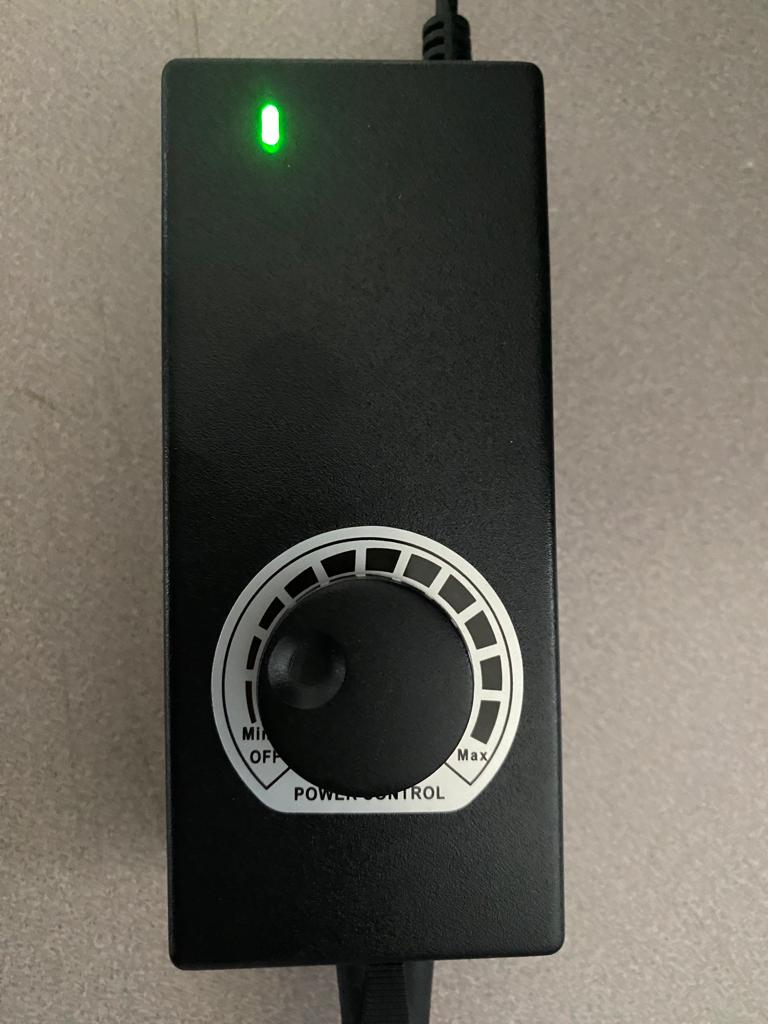
\includegraphics[width=0.4\textwidth]{dimer1}
\caption{Dimmer para el ajuste de la iluminación}
\label{dimmer}
\end{figure}

La cámara web cuenta con un sensor de tipo CMOS de 2-mega pixel \cite{camara}, obteniendo imágenes limpias y muy bien contrastadas.\\

El objetivo del proyecto, es el reconocer automáticamente ocho herramientas que son:

\begin{AutoMultiColItemize}
\item Martillo
\item Desarmador
\item Cinta de medir
\item Llave perica
\item Tijeras
\item Pinza de punta
\item Pinza eléctricas
\item Pinza de presión
\end{AutoMultiColItemize}

La toma de fotografias se realiza en un ambiente controlado como se muestra en la figura \ref{cubo}, ajustando la iluminación con un dimmer mostrado en la figura \ref{dimmer}.

\begin{figure}[h]
\centering
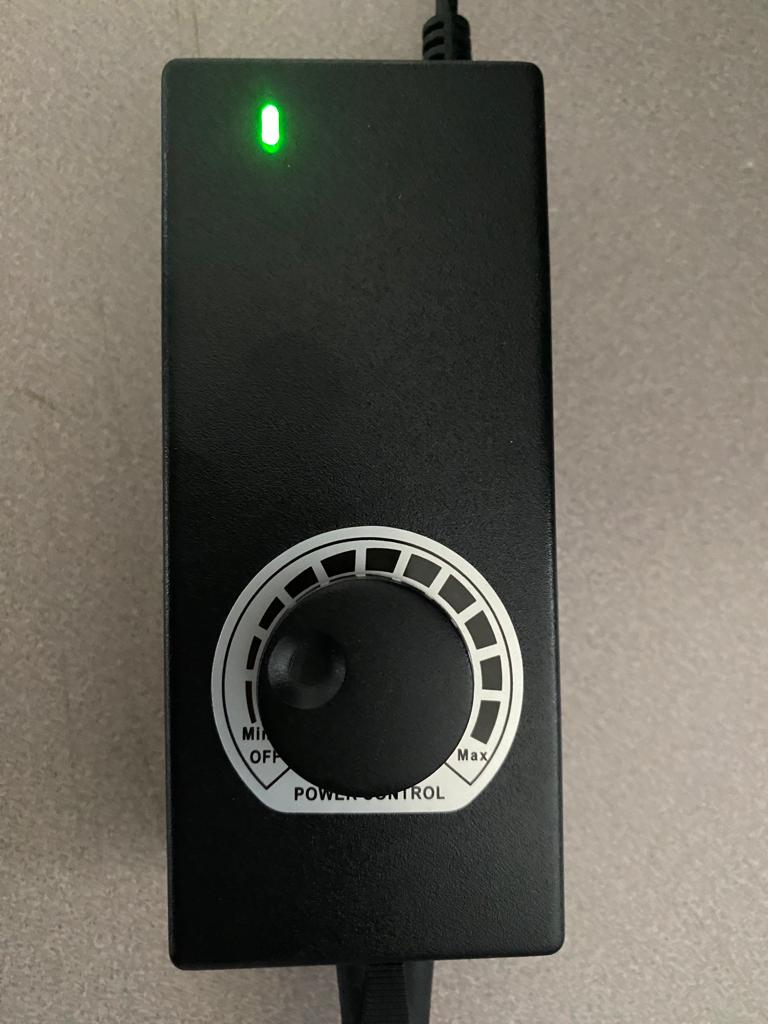
\includegraphics[width=0.4\textwidth]{dimer1}
\caption{Cubo para la adquisición de imágenes}
\label{cubo}
\end{figure}

Se usaron transformaciones geométricas para modificar la relación espacial entre píxeles en una imágen.\\

Usando propiedades que no deformen al objeto de interes como:

\begin{itemize}
\item Rotaciones
\item Traslaciones
\end{itemize}

Logrando crear imágenes artificiales, de modo tal que sirvan para el aumento del conjunto de imágenes.\\

\pagebreak
\section{Preprocesamiento}

Al contar con imágenes de buena calidad, sólo se mejoro el contraste para reducir las sombras que las herramientas pueden formar y lograr obtener el contorno que representa más la imagen a reconocer.\\

El mejoramiento como manipulación de una imagen tal que el resultado sea más útil que la imagen original para una aplicación particular.\\

Una transformación de intensidad modifica el constraste.\\

Ecualización del histograma.\\

No se tuvo que ecualizar ni mejorar por CLAHE, pero es bueno saber la existencia de estas tecnicas para crear sistemas y filtros sofisticados.\\

Modo de degradación de una imagen.\\

No se hizo uso de ningun filtro, buscando evitar el efecto de deslavado y poder detectar los bordes lo más puros posibles.\\

Pero el filtro de difusión anisotrópico puede considerarse en la implementación.\\

\section{Segmentación}

Se hacen pruebas con diversas técnicas de segmentación, optando por un resultado sencillo en base a operaciones morfologicas en base de una imagen de detección de bordes a partir de canny edges.\\

Contorno de una región\\

El contorno de una región conexa es el conjunto de pixeles que tienen al menos en pixel vecino que corresponde al fondo en 4 ó 8 adyacencia.\\

Buscar que tipo de etiquetado usa BWLABEL .- QUE ALGORITMO?\\

Etiquetado de regiones conexas\\


\pagebreak
\section{Extracción de caracteristicas}

El reconocimiento automático de objetos requiere calcular rasgos que describan propiedades fisicas de los objetos.\\

Un rasgo (atributo o caracteristica), es un valor numérico que cuantifica alguna propiedad de forma, textura, color, geometria, etc.

\begin{itemize}
\item Un rasgo debe ser discriminante, invariante, incorrelado y rápido de computar.
\item Los rasgos de forma generalmente se calculan a partir de la segmentación del objeto y se divide entre todos los pixeles de las regiones de interes.
\item Basados en región distribución de todos los pixeles.
\item Basados en contorno, variaciones a lo largo del contorno.
\end{itemize}

La extracción de caracteristicas que se utilizaron en el proyecto son las siguientes:

\begin{enumerate}
\item Rasgos geométricos básicos
\item Momentos de Hue
\item Cerco convexo
\item Esqueletización
\end{enumerate}

\subsubsection{Geométricas básicas}

\begin{itemize}
\item Redondez
\item Circularidad
\item Compacidad
\item Factor de forma
\end{itemize}

El área es el número total de pixeles que cubre la región del objeto.\\

El perimetro es la longitud del contorno del objeto. El resultado depende del tipo de conectividad que pueda tener.

\subsubsection{Rasgos basados en esqueleto}

\begin{itemize}
\item Puntos finales
\item Ramas
\item Número de pixles
\end{itemize}

\subsubsection{Momentos invariantes Hue}

Los momentos son proyecciones de una función sobre una base polinomial usados para medir la distribución de masa de un cuerpo.

\subsubsection{Cerco convexo}

Los momentos son proyecciones de una función sobre una base polinomial usados para medir la distribución de masa de un cuerpo.

\begin{itemize}
\item Solidez
\item Convexidad
\end{itemize}

\pagebreak
\section{Clasificación}

Etapas del reconocimiento de objetos en imagenes.

\begin{enumerate}
\item Sensado.- Capturar la imagen.
\item Preprocesamiento.- Mejorar la calidad de la imagen y segmentar los objetos de interes.
\item Extracción de caracteristicas.- Describir los objetos con rasgos cuantitativos discriminantes e invariantes.
\item Clasificación.- Asignar una etiqueta de clase a cada objeto.
\end{enumerate}

Obtener un vector de patrones.

Para el proyecto se consideran ocho clases sindo representadas por los objetos siguientes:

\begin{enumerate}
\item Cinta de medir
\item Desarmador
\item Martillo
\item Pinza electrica
\item Pinza de presión
\item Pinza de punta
\item Perica
\item Tijeras
\end{enumerate}

En este proyecto se usa el método de datos de entrenamiento que son vectores de patrones asociados a una etiqueta de clase (x,y) con $y \in \Omega = {w_{1},...,w_{c}}$\\

MOSTRAR EN DIAGRAMA DE LOS PROCEOS PARA LA CLASIFICACION\\

La selección del algoritmo de clasificación debe tener las siguientes cualidades.

\begin{itemize}
\item Generación de fronteras de decisión no lineales.
\item Clasificación en más de dos clases (multiclases).
\item Entrenamiento en un tiempo de cómputo razonable. 
\end{itemize}

Se elige el clasificador k-nn de vecinos más cercanos por su simpleza.

\newpage
\section{Resultados}

\begin{figure}[h]
  \centering
  \begin{subfigure}{0.45\linewidth}
    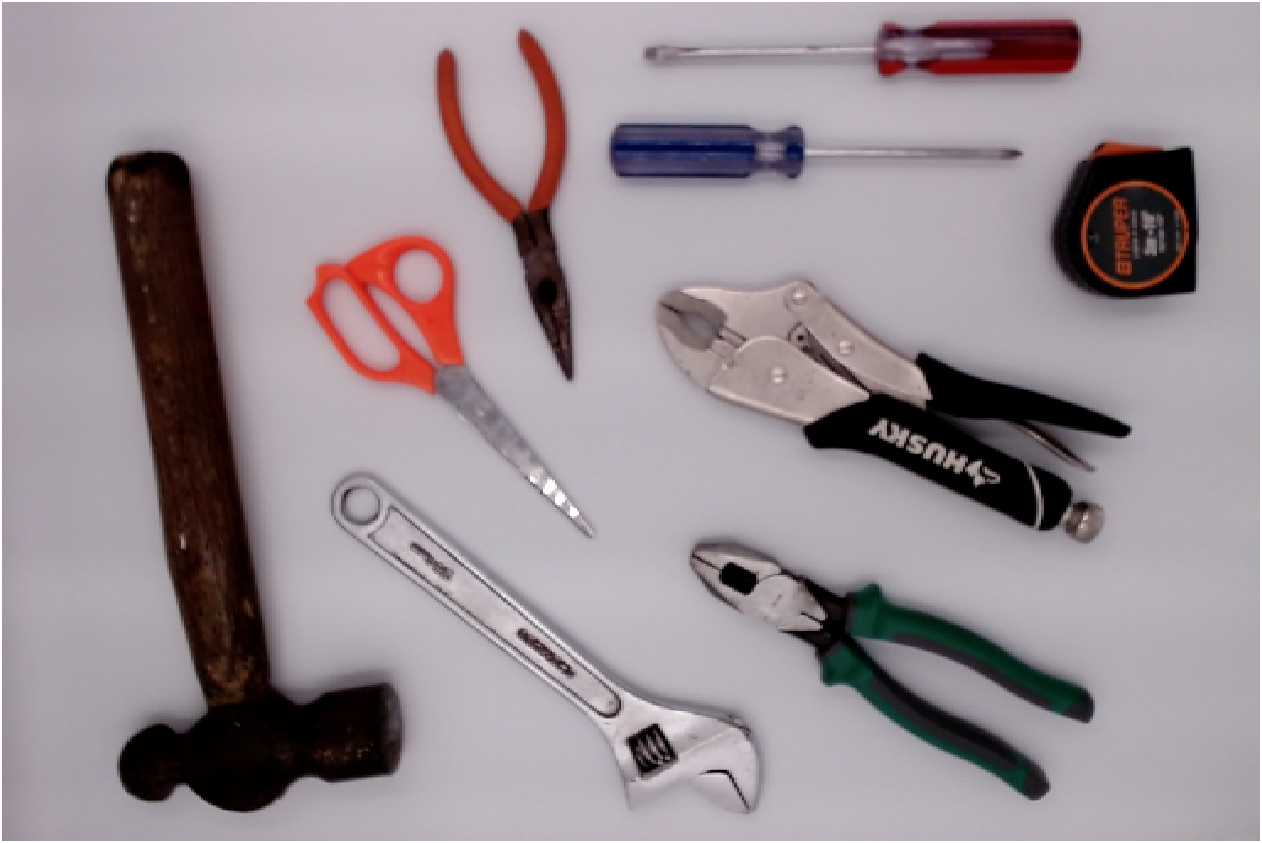
\includegraphics[width=\linewidth]{paso1} 
    \caption{}
    \label{fig:1a}
  \end{subfigure}\hfill
  \begin{subfigure}{0.45\linewidth}
    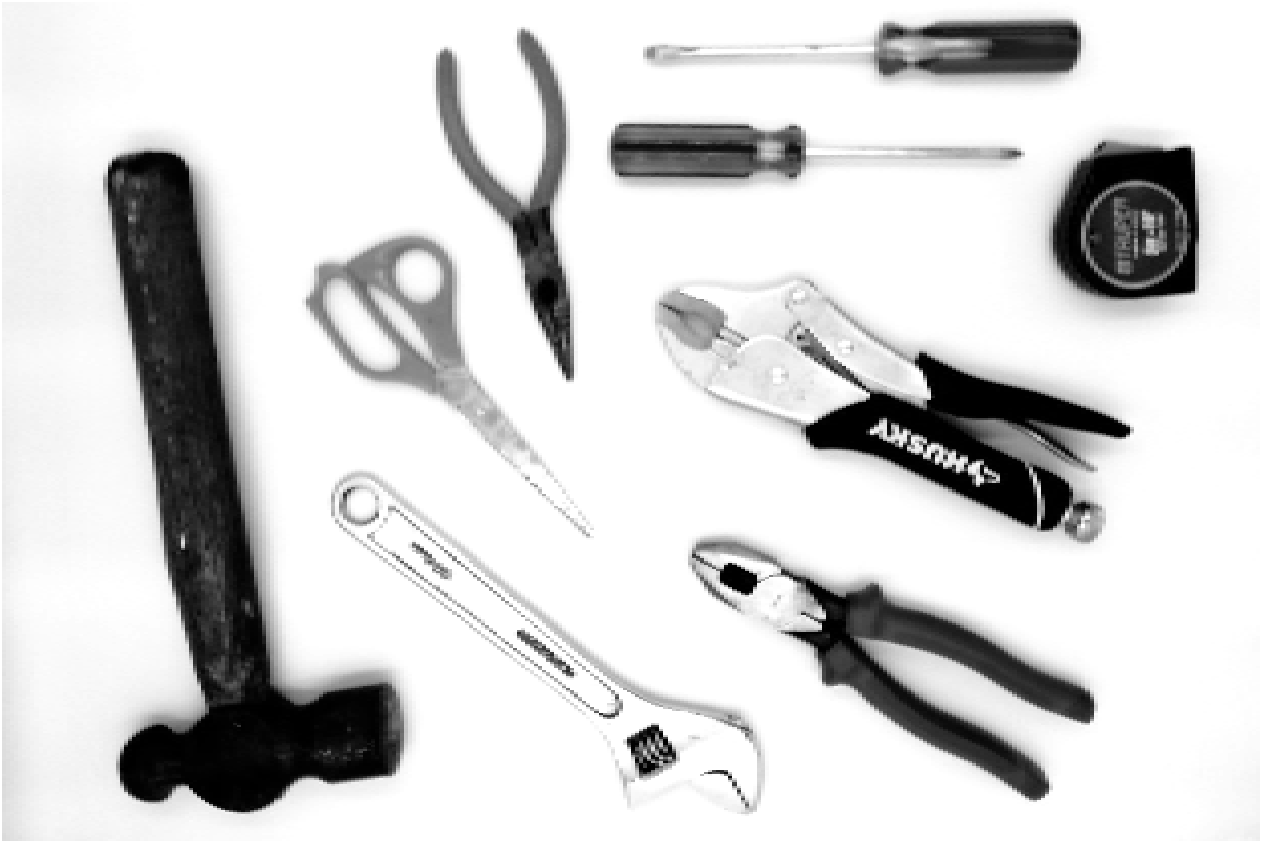
\includegraphics[width=\linewidth]{paso2}
    \caption{}
    \label{fig:1a}
  \end{subfigure}
  
  \begin{subfigure}{0.45\linewidth}
    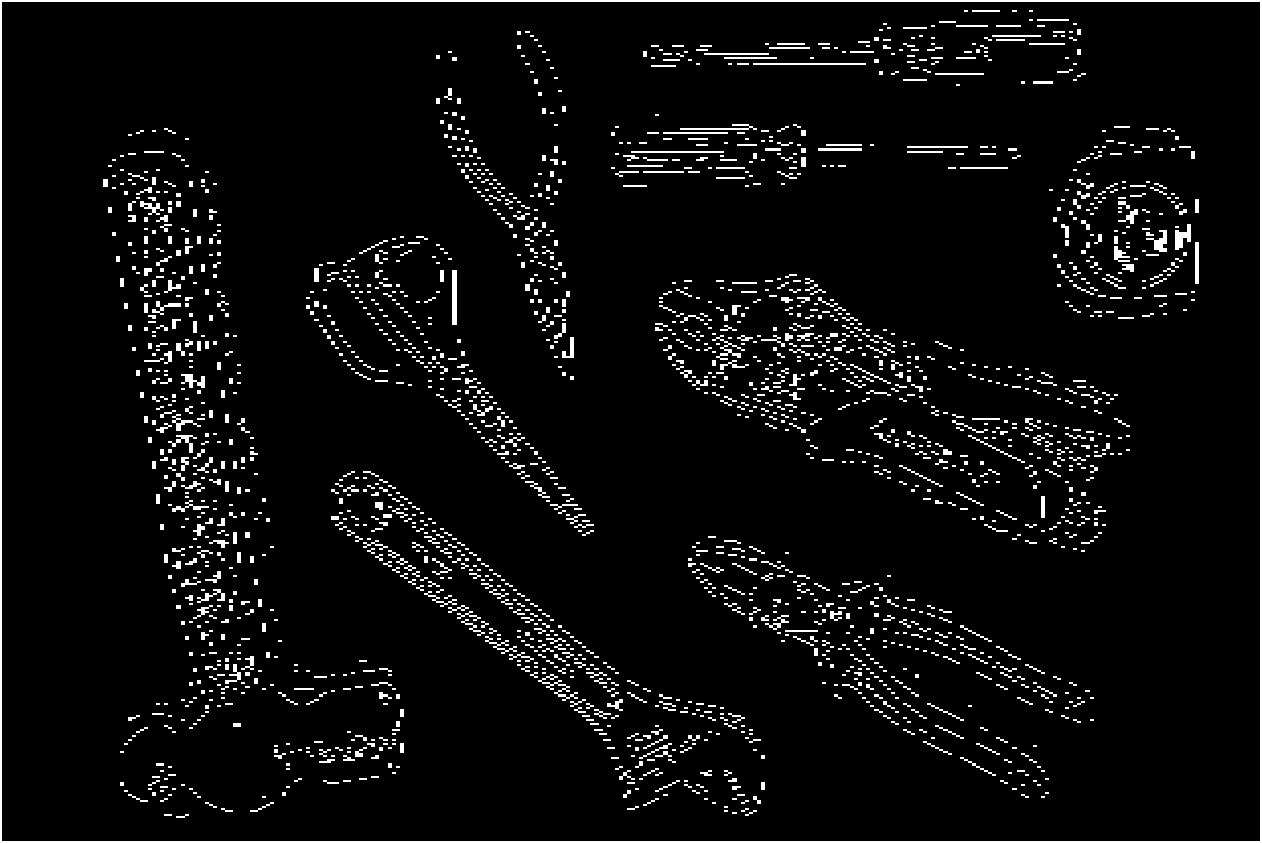
\includegraphics[width=\linewidth]{paso3}
    \caption{}
    \label{fig:1a}
  \end{subfigure}\hfill
  \begin{subfigure}{0.45\linewidth}
    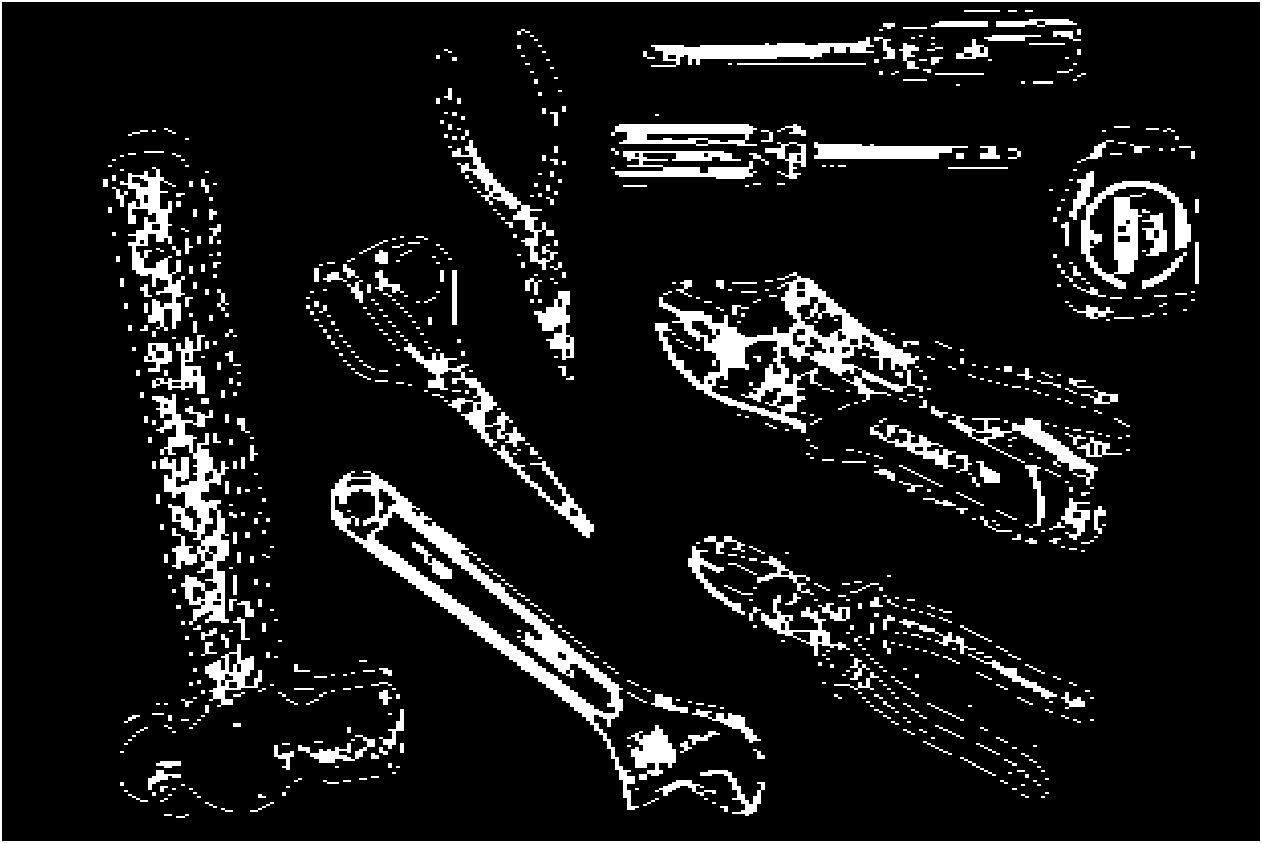
\includegraphics[width=\linewidth]{paso4}
    \caption{}
    \label{fig:1a}
  \end{subfigure}
  \caption{My composed figure}
  \label{fig:1}
\end{figure}

\begin{figure}[h]
  \centering
  \begin{subfigure}{0.45\linewidth}
    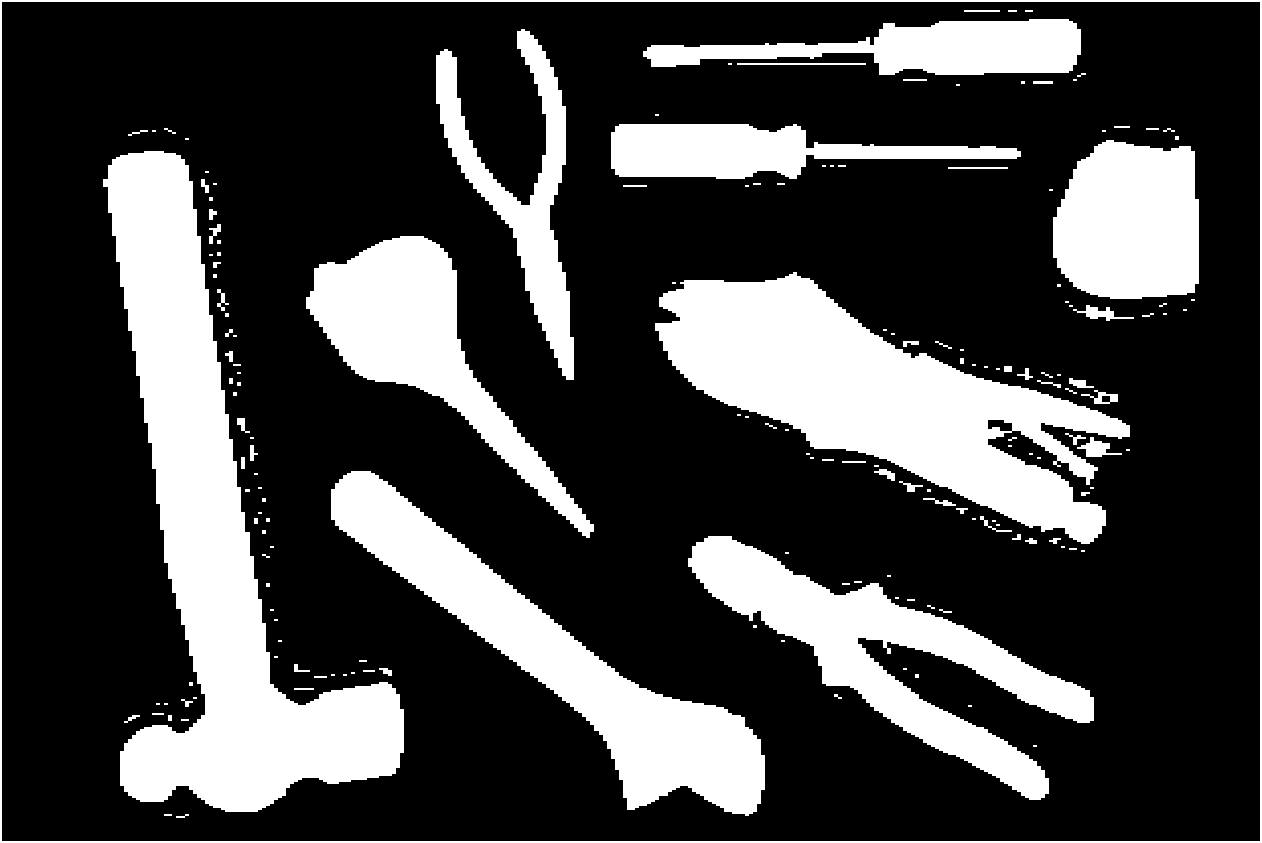
\includegraphics[width=\linewidth]{paso5} 
    \caption{}
    \label{fig:1a}
  \end{subfigure}\hfill
  \begin{subfigure}{0.45\linewidth}
    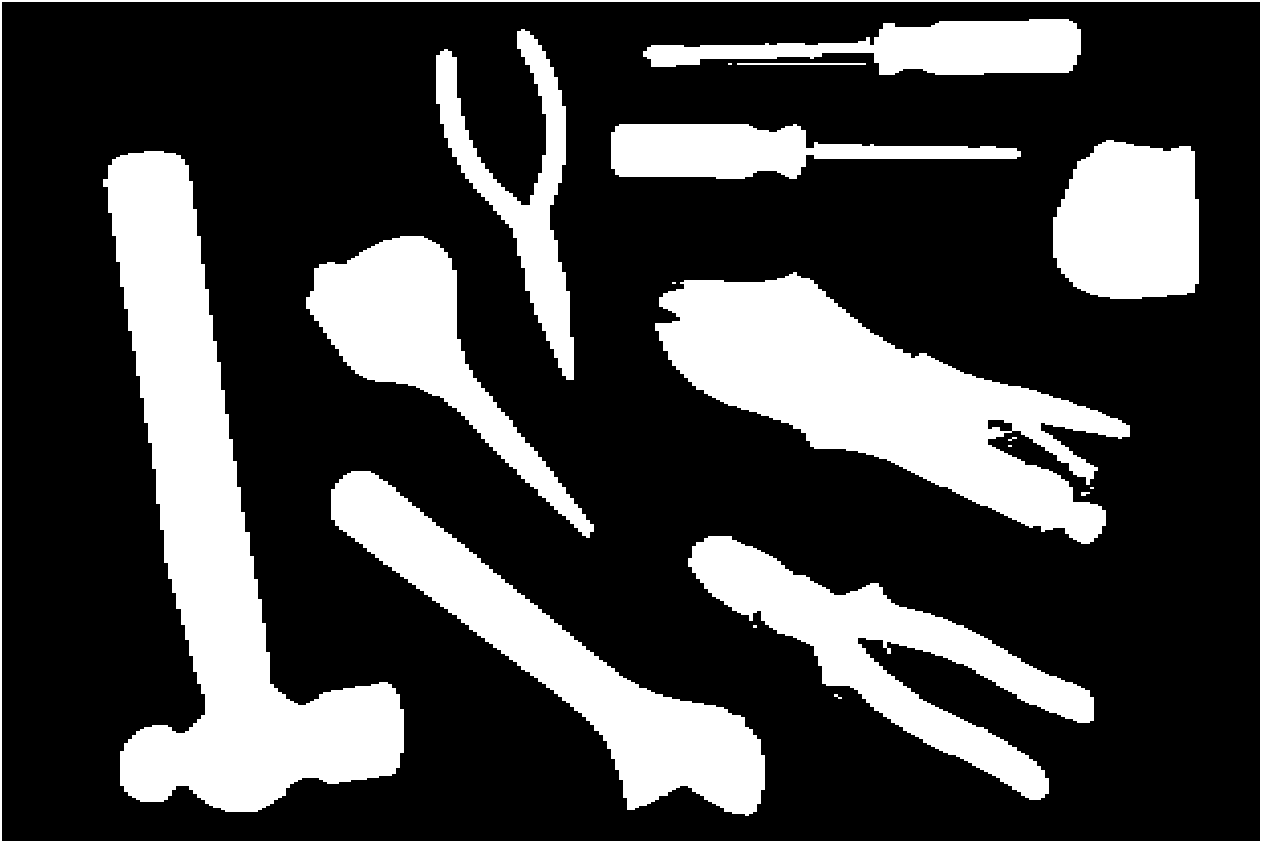
\includegraphics[width=\linewidth]{paso6}
    \caption{}
    \label{fig:1a}
  \end{subfigure}
  
  \begin{subfigure}{0.45\linewidth}
    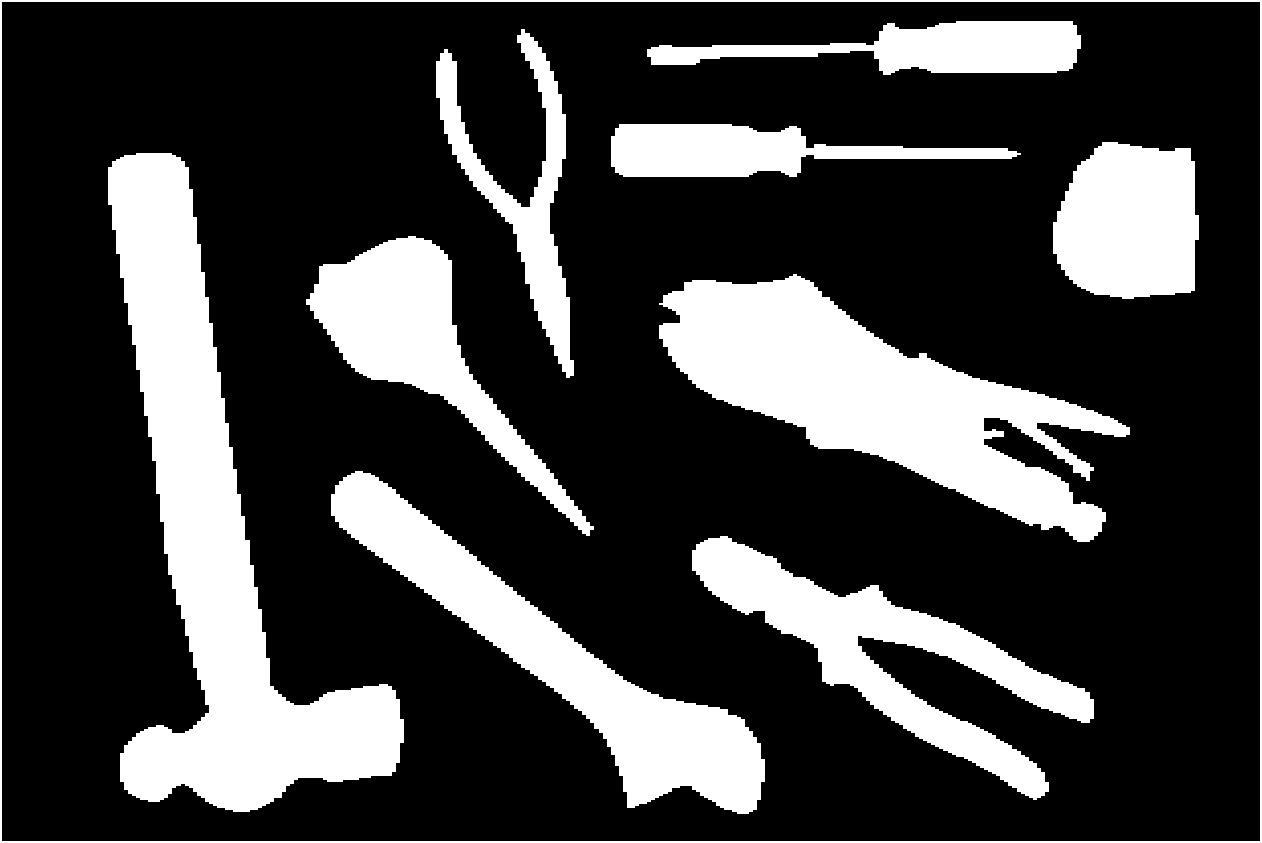
\includegraphics[width=\linewidth]{paso9}
    \caption{}
    \label{fig:1a}
  \end{subfigure}\hfill
  \begin{subfigure}{0.45\linewidth}
    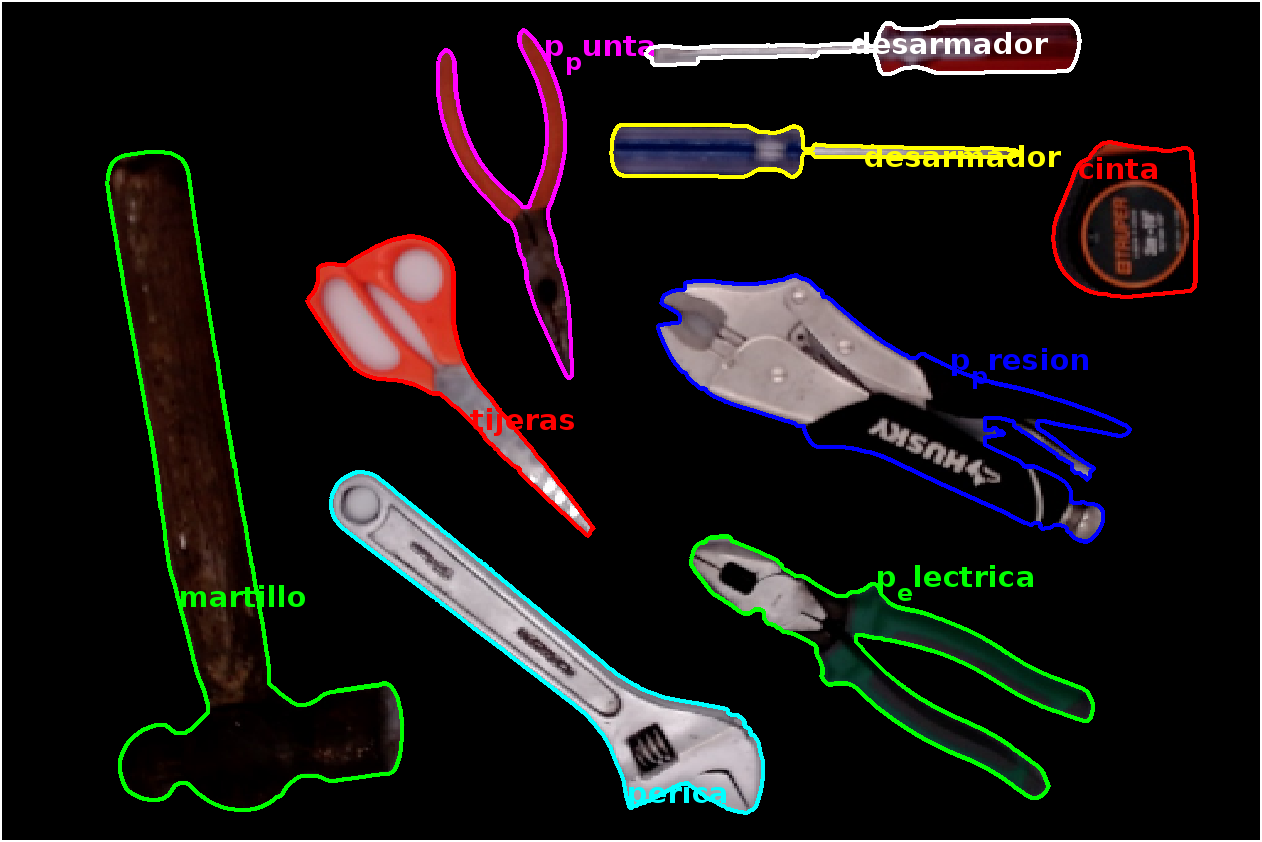
\includegraphics[width=\linewidth]{paso10}
    \caption{}
    \label{fig:1a}
  \end{subfigure}
  \caption{My composed figure}
  \label{fig:1}
\end{figure}


Dentro de las imagenes, la similitud de esqueletos entre la cinta, la llave perica, tijera, pinzas de punta y electrica que tienen formas similares.

La mayoria de desarmadores no tiene ramas y tiene dos puntos finales, lo que lo confunde con una cinta al solo considerar las ramas y los puntos terminales se tiene una exactitud del 20\%, mientras al agregar el num de pixeles crece al 78\%, agregando más información como el área y perimetro la probabilidad de acierto crece aún más, presentandose valores arriba del 90\%.
\pagebreak

\section{Apendice}

\subsection{Script de rasgos}

La obtención de rasgos se realizo mediante un script que itera entre todas las carpetas de las imágenes, haciendo rotaciones y traslaciones aleatorias, buscando mantener la imagen, por lo que se le añade un efecto para que el fondo se replique


\begin{lstlisting}[style=Matlab-editor, caption=Script de rasgos]
%% Sample Matlab code
!mv test.txt test2.txt
A = [1, 2, 3;... foo
     4, 5, 6];
s = 'abcd';
for k = 1:4
  Disp(s(k)) % bar
end
%{
create row vector x, then reverse it
%}
x = linspace(0,1,101);
y = x(end:-1:1);
\end{lstlisting}


\subsection{Script de data aumentation}

We did some experiments \ldots

\begin{lstlisting}[style=Matlab-editor, caption=Python example]
%% Sample Matlab code
!mv test.txt test2.txt
A = [1, 2, 3;... foo
     4, 5, 6];
s = 'abcd';
for k = 1:4
  Disp(s(k)) % bar
end
%{
create row vector x, then reverse it
%}
x = linspace(0,1,101);
y = x(end:-1:1);
\end{lstlisting}

\pagebreak

\section{Experimentando en python}

\begin{lstlisting}[language=Python, caption=experimentación python]
import numpy as np
    
def incmatrix(genl1,genl2):
    m = len(genl1)
    n = len(genl2)
    M = None #to become the incidence matrix
    VT = np.zeros((n*m,1), int)  #dummy variable
    
    #compute the bitwise xor matrix
    M1 = bitxormatrix(genl1)
    M2 = np.triu(bitxormatrix(genl2),1) 

    for i in range(m-1):
        for j in range(i+1, m):
            [r,c] = np.where(M2 == M1[i,j])
            for k in range(len(r)):
                VT[(i)*n + r[k]] = 1;
                VT[(i)*n + c[k]] = 1;
                VT[(j)*n + r[k]] = 1;
                VT[(j)*n + c[k]] = 1;
                
                if M is None:
                    M = np.copy(VT)
                else:
                    M = np.concatenate((M, VT), 1)
                
                VT = np.zeros((n*m,1), int)
    
    return M
\end{lstlisting}

\begin{lstlisting}[language=Python, caption=Python example]
import numpy as np
    
def incmatrix(genl1,genl2):
    m = len(genl1)
    n = len(genl2)
    M = None #to become the incidence matrix
    VT = np.zeros((n*m,1), int)  #dummy variable
    
    #compute the bitwise xor matrix
    M1 = bitxormatrix(genl1)
    M2 = np.triu(bitxormatrix(genl2),1) 

    for i in range(m-1):
        for j in range(i+1, m):
            [r,c] = np.where(M2 == M1[i,j])
            for k in range(len(r)):
                VT[(i)*n + r[k]] = 1;
                VT[(i)*n + c[k]] = 1;
                VT[(j)*n + r[k]] = 1;
                VT[(j)*n + c[k]] = 1;
                
                if M is None:
                    M = np.copy(VT)
                else:
                    M = np.concatenate((M, VT), 1)
                
                VT = np.zeros((n*m,1), int)
    
    return M
\end{lstlisting}

\pagebreak

\section{Conclusiones}

Estudios tempranos de Inteligencia Artificial buscaban duplicar los pensamientos humanos, pero ahora los estudios recientes muestran la tendencia en replicar el resultado y las computadoras actuan como sistemas expertos.\\

Las computadoras son dispositivos simbolicos capaces de manipular cualquier tipo de simbolos siendo los numeros una clase importante, pero las computadoras son más generales que eso. Sabemos de la generalidad de la computación desde los tiempos de Alan Touring en los 1930's y se tienen intuiciones que Babbage tuvo también estudios que fueron afirmados por Ada Lovelace, en 1842 Ada Lovelace escribió sobre la ingenieria analitica de Babbage que buscaba unir el mundo mecanico con el mundo de las cosas abstractas, en la psicologia moderna es llamado The physical symbol system hypothesis y son las bases en que la Inteligencia Artificial funciona.\\

La Inteligencia Artificial como ciencia emplea el uso de computadoras para procesar conocimientos simbolicos usando metodos de inferencias logicas, en otras palabras, nos referimos a inferencia y no calculos que se piensa en el sentido tradicional, hablamos de conocimiento y no numeros como en la forma tradicional.\\
Al poner conocimiento en programas computacionales que para los humanos nos es fácil o a veces un reto intelectual y el conocimiento que le pasamos es representativo en cierta forma particular.\\

Por otra parte, los sistemas expertos basados en conocimientos son aplicables en cualquier  área en que sea especializado el conocimiento y sea rutinario la toma de desiciones, estrategias para resolver problemas, diagnosticos, .. etc.\\
Siendo de gran ayuda en un gran rango de aplicaciones, el \textbf{conocimiento medico}, en clasificación de un experto, puede estar reflejado con el funcionamiento de una red neuronal.\\

Para algun diagnostico médico ó segmentadores más fáciles, pero igual de complicados como la segmentación en imágenes para la creación de sistemas autonomos.\\

Programas que se puedan ejecutar en cualquier computadora o dispositivo que permita la ejecución de código multiplataforma como python ó C++, que tienen capacidades altas de manipulación simbolica, la toma de desiciones es primordial en una inteligencia basada en conocimiento y esa manipulación simbolica es necesaria.

\pagebreak
\bibliographystyle{abbrv}
\bibliography{referencias}  % need to put bibtex references in references.bib 
\end{document}
